\documentclass[a4paper]{article}
\usepackage[pdftex]{graphicx}
\usepackage[utf8]{inputenc}
\usepackage{enumerate}
\usepackage{amssymb}
\usepackage{tikz}
\usepackage{href-ul}
\hypersetup{
	colorlinks=true,
	linkcolor=blue,
	urlcolor=blue}
\usepackage{geometry}
\geometry{a4paper, top=15mm, left=15mm, right=15mm, bottom=15mm,
	headsep=10mm, footskip=12mm}

\begin{document}
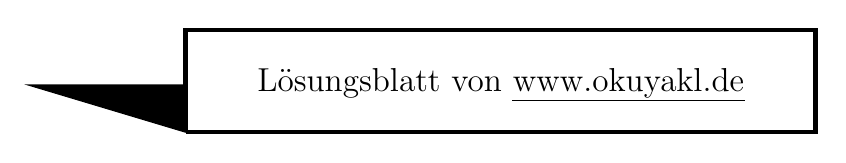
\begin{tikzpicture}(10,3)
	\draw[ultra thick](2,0) --(10,0) -- (10,1.3) --(2,1.3) -- (2,0);
	\draw[fill=black](2,0)-- (0,.6) -- (2,.6) -- (2,0);
	\node at (6,.6) {\large Lösungsblatt von \href{https://www.okuyakl.de}{www.okuyakl.de}};
\end{tikzpicture}
\vspace{0.5 cm}

\noindent{\bf Aufgabe 1.}\\
\renewcommand{\arraystretch}{1}
\begin{tabular}{lll}
	a) $\left(\begin{array}{c} -4 \\11 \\ 14\end{array} \right) $ & b) $\left(\begin{array}{c} 0 \\ 2\\ -11\end{array} \right) $ & c) $\left(\begin{array}{c} 11 \\-11 \\ -4\end{array} \right) $
\end{tabular}

\noindent{\bf Aufgabe 2.}\\
\renewcommand{\arraystretch}{1}
\begin{tabular}{lll}
	a) $\vec{x}=\left(\begin{array}{c} 9 \\10 \\ -7\end{array} \right) $ &
	b) $\vec{x}=\left(\begin{array}{c} -0,5 \\9,5 \\ -1,5\end{array} \right) $ &
	c) $\vec{x}=\left(\begin{array}{c} 1 \\4 \\ -12\end{array} \right) $ 
\end{tabular}

\noindent{\bf Aufgabe 3.}\\
\renewcommand{\arraystretch}{2}
\begin{tabular}{llll}
	a) $M(1|-2|5) $ & b) $M(6,5|5|0,5) $ & c) $D(7|1|4) $ & d) $G(-14|2|-4) $ 
\end{tabular}

\begin{minipage}{0.5\textwidth}
	\noindent{\bf Aufgabe 4.}\\
	
	$$\overrightarrow{OD_1}=\overrightarrow{OC}+ \overrightarrow{BA} \qquad \Rightarrow	D_1(12|-5|6) $$
	$$\overrightarrow{OD_2}=\overrightarrow{OC}+ \overrightarrow{AB} \qquad \Rightarrow	D_2(4|-1|-6) $$
	$$\overrightarrow{OD_3}=\overrightarrow{OA}+ \overrightarrow{CB} \qquad \Rightarrow D_3(-6|9|6) $$
\end{minipage}
\begin{minipage}{0.5\textwidth}
	\includegraphics[width=6 cm]{parad109}
\end{minipage}

\noindent{\bf Aufgabe 5.}\\
$$ \overrightarrow{OC}=\overrightarrow{OA}+ 2\cdot \overrightarrow{AM} \qquad \Rightarrow	C(6|-6|-2) $$
$$\overrightarrow{OD}=\overrightarrow{OB}+ 2\cdot \overrightarrow{BM} \qquad \Rightarrow	D(0|-1|-4) $$

\noindent{\bf Aufgabe 6.}\\
$$\overrightarrow{OT}=\overrightarrow{OA}+ {1\over 3}\cdot \overrightarrow{AB} \qquad \Rightarrow	T(1|-3|6) $$
$$\overrightarrow{OR}=\overrightarrow{OA}+ {2\over 3}\cdot \overrightarrow{AB} \qquad \Rightarrow	T(4|-7|11) $$

\noindent{\bf Aufgabe 7.}\\
\renewcommand{\arraystretch}{2}
\begin{tabular}{lll}
	a) $a=4;\quad b=-9 $ & b) $u=-6;\quad v=4 $ & c) $k=-6;\quad m=1 $ 
\end{tabular}

\noindent{\bf Aufgabe 8.}\\
\renewcommand{\arraystretch}{2}
\begin{tabular}{lllll}
	a) $a=\pm 2$ & b) $t=\pm 3$ & c) $s=\pm 3$ & d) $r=0$ & e) $t=\pm 2$ 
\end{tabular}

\noindent{\bf Aufgabe 9.}\\
\renewcommand{\arraystretch}{2}
\begin{tabular}{lll}
	a) $v=-3$ & b) $u=-2,5$ & c) $t_1=5;\quad t_2=-5$
\end{tabular}

\noindent{\bf Aufgabe 10.}\\
\begin{enumerate}[a)]
	\item $\alpha=83,4^\circ; \quad \beta=59,8^\circ;\quad \gamma=36,8^\circ$
	\item $\alpha=\beta=\gamma=60^\circ$
\end{enumerate}


\begin{center}
	\includegraphics[width=7 cm]{../../viecher/endcomic.pdf}
	
	Hier geht es zurück zum \href{https://www.okuyakl.de/math/m11skaL109/aa109.pdf}{Aufgabenblatt}
\end{center}

\end{document}
